\documentclass[12pt,a4paper]{article}

\title{P-unit model by Henriette Walz \& Alexander Ott}
\author{Alexandra Rudnaya, Jan Grewe, Jan Benda}
\date{June 2022}

%%%%% layout %%%%%%%%%%%%%%%%%%%%%%%%%%%%%%%%%%%%%%%%%%%%%%%%%%%%%%%%%%%%%%%%
\usepackage[left=20mm,right=20mm,top=20mm,bottom=20mm]{geometry}
%\setcounter{secnumdepth}{-1}

%%%%% units %%%%%%%%%%%%%%%%%%%%%%%%%%%%%%%%%%%%%%%%%%%%%%%%%%%%%%%%%%%%%%%%%
\usepackage[mediumspace,mediumqspace,Gray,amssymb]{SIunits}      % \ohm, \micro

%%%%% math %%%%%%%%%%%%%%%%%%%%%%%%%%%%%%%%%%%%%%%%%%%%%%%%%%%
\usepackage{textcomp}
\usepackage{array}
\usepackage{amsmath}
\usepackage{amssymb}
\usepackage{graphicx}

%%%%% equation references %%%%%%%%%%%%%%%%%%%%%%%%%%%%%%%%%%%%%%%%%%%%%%%%%%%
\renewcommand{\eqref}[1]{(\ref{#1})}
\newcommand{\eqn}{Eq.}
\newcommand{\Eqn}{Eq.}
\newcommand{\eqns}{Eqs.}
\newcommand{\Eqns}{Eqs.}
\newcommand{\eqnref}[1]{\eqn~\eqref{#1}}
\newcommand{\Eqnref}[1]{\Eqn~\eqref{#1}}
\newcommand{\eqnsref}[1]{\eqns~\eqref{#1}}
\newcommand{\Eqnsref}[1]{\Eqns~\eqref{#1}}
 
%%%%% hyperef %%%%%%%%%%%%%%%%%%%%%%%%%%%%%%%%%%%%%%%%%%%%%%%%%%%%%%%%%%%%%%%
\usepackage{xcolor}
\usepackage[breaklinks=true,colorlinks=true,citecolor=blue!30!black,urlcolor=blue!30!black,linkcolor=blue!30!black]{hyperref}

%%%%% notes %%%%%%%%%%%%%%%%%%%%%%%%%%%%%%%%%%%%%%%%%%%%%%%%%%%%%%%%%%%%%%%%
\newcommand{\note}[2][]{\textbf{[#1: #2]}}

%%%%%%%%%%%%%%%%%%%%%%%%%%%%%%%%%%%%%%%%%%%%%%%%%%%%%%%%%%%%%%%%%%%%%%%%%%%%%
%%%%%%%%%%%%%%%%%%%%%%%%%%%%%%%%%%%%%%%%%%%%%%%%%%%%%%%%%%%%%%%%%%%%%%%%%%%%%
\begin{document}

\maketitle


\section{The model}

The input into the P-unit model, $x(t)$, is
\begin{itemize}
\item the fish's own EOD
  \begin{equation}
    \label{eod}
    x(t) = x_{EOD}(t) = \cos(2\pi f_{EOD} t)
  \end{equation}
  with EOD frequency $f_{EOD}$ and amplitude normalized to one.
\item the EOD multiplied with an amplitude modulation $AM(t)$:
  \begin{equation}
    \label{am}
    x(t) = (1+AM(t)) \cos(2\pi f_{EOD} t)
  \end{equation}
  For a random amplitude modulaten ($AM(t) = RAM(t)$) random numbers
  are drawn for each frequency up to $f_{EOD}/2$ in Fourier
  space. After backtransformation the resulting signal is scaled to
  the desired standard deviation relative to the EOD carrier.
\item a superposition of two EODs
  \begin{equation}
    \label{beat}
    x(t) = x_{EOD}(t) + x_{EOD1}(t) = \cos(2\pi f_{EOD} t) + \alpha_1 \cos(2\pi f_{EOD1} t)
  \end{equation}
  with the EOD of the second fish having frequency $f_{EOD1}$ and amplitude $\alpha_1$ relative to the amplitude of the receiving fish.
\item a superposition of many EODs
  \begin{equation}
    \label{multibeat}
    x(t) = x_{EOD}(t) + \sum_{i=1}^{n} x_{EODi}(t) = \cos(2\pi f_{EOD} t) + \sum_{i=1}^{n} \alpha_i \cos(2\pi f_{EODi} t) \; .
  \end{equation}
  For $n=2$ this is our cocktail-party problem.  
\end{itemize}
The input $x(t)$ is a normalized EOD and thus is unitless.

First, the input $x(t)$, is thresholded potentially at the synapse between the receptor cells and the afferent, and then low-pass filtered  with time constant $\tau_{d}$ by the afferent's dendrite:
\begin{equation}
  \label{dendrite}
  \tau_{d} \frac{d V_{d}}{d t} = -V_{d}+  \lfloor x(t) \rfloor_{0}^{p}
\end{equation}
Because the input is unitless, the dendritic voltage is unitless, too. $\lfloor x(t) \rfloor_{0}$ denotes the threshold operation that sets negative values to zero:
\begin{equation}
  \label{threshold}
  \lfloor x(t) \rfloor_0 = \left\{ \begin{array}{rcl} x(t) & ; & x(t) \ge 0 \\ 0 & ; & x(t) < 0 \end{array} \right.
\end{equation}
Usually the exponent $p$ is set to one (pure threshold). In our advanced models $p$ is set to three in order to reproduce responses to beats with difference frequencies above half of the EOD frequency.

This thresholding and low-pass filtering extracts the amplitude modulation of the input $x(t)$. The dendritic voltage $V_d(t)$ is the input to a leaky integrate-and-fire (LIF) model
\begin{equation}
  \label{LIF}
  \tau_{m} \frac{d V_{m}}{d t}  = - V_{m} + \mu + \alpha V_{d} - A + \sqrt{2D}\xi(t)
\end{equation}
where $\tau_{m}$ the membrane time constant, $\mu$ a fixed bias current, $\alpha$ a scaling factor for $V_{d}$, and $\sqrt{2D}\xi(t)$ a white noise of strength $D$. All terms in the LIF are unitless.

The adaptation current $A$ follows
\begin{equation}
  \label{adaptation}
  \tau_{A} \frac{d A}{d t} = - A
\end{equation}
with adaptation time constant $\tau_A$.

Whenever the membrane voltage $V_m(t)$ crosses the threshold $\theta=1$ a spike is generated, $V_{m}(t)$ is reset to $0$, the adaptation current is incremented by $\Delta A$, and integration of $V_m(t)$ is paused for the duration of a refractory period $t_{ref}$:
\begin{equation}
  \label{spikethresh}
  V_m(t) \ge \theta \; : \left\{ \begin{array}{rcl} V_m & \mapsto & 0 \\ A  & \mapsto & A + \Delta A/\tau_A \end{array} \right.
\end{equation}


\section{Parameter values}

\note[JB]{Sascha, list all parameters (table or itemize) plus time step of the model with typical values and the right (time) units}


\begin{table}[h!]
  \begin{center}
    \caption{Model parameters.}
    \label{tab:table1}
    \begin{tabular}{l|c|l}
      
      parameter & explanation & median parameter \\
      \hline
      $\alpha$  & stimulus scaling factor &  90.533695\\
      $\tau_{m}$  & membrane time constant &  0.001847\,s\\       
      $\mu$  & bias current &  -17.1875\\      
      $\sqrt{2D}$  & noise strength &  0.01848 \\      
      $\tau_{A}$  & adaption time constant &  0.111759\,s\\      
      $\Delta A$  & adaption strength &  0.122197\\      
      $\tau_{d}$  & time constant of dendritic low-pass filter &  0.002463\,s\\      
      $t_{ref}$  & absolute refractory period &  0.000965\,s\\     
	  $\Delta t$  & time step &  0.00005\,s\\           
    \end{tabular}
  \end{center}
\end{table}
\begin{figure*}[tp]
  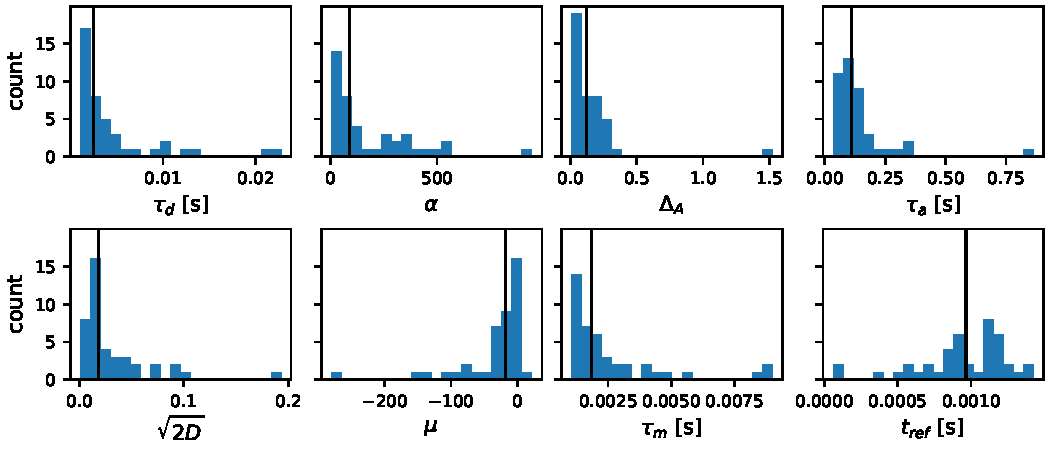
\includegraphics{parameter_distribution}
  \caption{\label{parameter_distribution} The distribution of the model parameters.
}
\end{figure*}





\section{Numerical implementation}




\note[JB]{Sascha: This is Alexander Ott's code from the git repository, right?}
\note[SR]{Yes that is correct.}
The ODEs are integrated by the Euler forward method with time-step $\Delta t$.

For the intrinsic noise of the model $\xi(t)$ in each time step $i$ a random number is drawn from a normal distribution $\mathcal{N}(0,\,1)$ with zero mean and standard deviation of one. This number is multiplied with $\sqrt{2D}$ and divided by $\sqrt{\Delta t}$:
\begin{equation}
  \label{LIFintegration}
  V_{m_{i+1}}  = V_{m_i} + \left(-V_{m_i} + \mu + \alpha V_{d_i} - A_i + \sqrt{\frac{2D}{\Delta t}}\mathcal{N}(0,\,1)_i\right) \frac{\Delta t}{\tau_m}
\end{equation}
\note[JB]{Benjamin: wir haben das Rauschen innerhalb der Klammer. Damit ist zwar das $\sqrt{\Delta t}$ richtig, aber wir teilen noch durch $\tau_m$. Damit sind effektiv unsere $D$ Werte andere als wenn wir den Rauschterm ausserhalb der Klammer haetten (so machst du das glaube ich immer).}

The noise strength values from the table in fact equal $\sqrt{2D}$ and not $D$.

\note[JB]{we need to clean up that noise issue}
\note[SR]{Mascha hat mir jetzt auch ein PDF File geschickt wie die das machen. Sollen wir einfach unsere alles an deren Vorgehen anpassen?}

\end{document}
